\chapter{Objetivos y metodología}\label{cap.objetivos}
En este capítulo se expondrá de manera detallada el objetivo principal de este proyecto así como la metodología utilizada para su desarrollo. También se incluirá un plan de trabajo donde se explican las diferentes etapas seguidas en su realización.

\section{Objetivos}

El objetivo principal de este trabajo es llevar a cabo dos nuevas prácticas para la plataforma JdeRobot-Academy. Para cada práctica se creará el enunciado, la infraestructura necesaria en Gazebo, un nodo académico donde los estudiantes empotrarán su código y una solución tentativa.  \\

El objetivo de la práctica ``Coche autónomo negocia un cruce'' es conseguir que un coche autónomo sea capaz de reconocer una señal de stop situada a lo largo de una carretera, gracias a la cámara que lleva situada en el techo, y después, frene. Además, tiene que ser capaz de reconocer si se acercan otros coches y en caso negativo volver a arrancar. Y por último, tiene que hacer un giro a la izquierda o a la derecha de manera aleatoria. \\

En la práctica ``Aspiradora autónoma con autolocalización'', el objetivo es lograr que un robot aspirador sea capaz de limpiar la mayor superficie posible de un apartamento en un tiempo limitado. Para ello, el alumno hará uso de la capacidad de autolocalización de la aspiradora y del mapa de la casa.\\

Uno de los requisitos de las prácticas es que los alumnos sólo tengan que concentrarse en la parte de programación de robots no en funcionalidades auxiliares necesarias, como el interfaz gráfico o el mecanismo particular de acceso a sensores y actuadores. El nodo académico de cada práctica debe resolver eso y ofrecérselo de manera sencilla al estudiante. Además, gracias a la realización de estas prácticas el alumno adquirirá tanto conocimientos sobre programación de Python en robótica como conocimientos relacionados con el tratamiento digital de la imagen y la toma de decisiones.


\section{Metodología}

El desarrollo de trabajo que se ha seguido es el modelo en espiral. Este modelo consiste en una serie de ciclos o iteraciones que se repiten en forma de espiral como se muestra en la Figura~\ref{fig.espiral}.

\begin{figure}[H]
  \begin{center}
    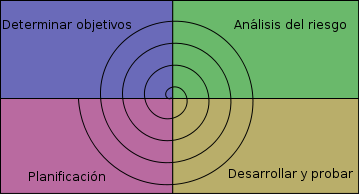
\includegraphics[width=0.6\textwidth]{figures/Objetivos/espiral.png}
		\caption{Metodología en espiral}
		\label{fig.espiral}
		\end{center}
\end{figure}

Cada ciclo consta de cuatro fases:
\begin{itemize}
	\item Determinar objetivos que se deben de llevar a cabo para que una vez completados se pueda dar por finalizado el ciclo.

	\item Análisis del riesgo: se evalúa qué problemas es posible encontrarse al empezar el desarrollo.

	\item Desarrollar y probar: en la tercera fase, una vez evaluados los riesgos, se procede al propio desarrollo del trabajo realizando distintas pruebas para conseguir el mejor resultado.

	\item Planificación: en esta última fase se valoran los resultados obtenidos y se planifican los siguientes etapas del proyecto.
\end{itemize}

No existe un número fijo de iteraciones, deben de llevarse a cabo tantas como sean necesarias hasta completar el trabajo. \\

Una ventaja del modelo de espiral en la ingeniería de software es que se adapta a cualquier número de cambios que pueden ocurrir durante cualquier fase del proyecto, permitiendo minimizar los riesgos y una buena evolución del trabajo. \\

Se han ido acordando reuniones semanales con el tutor. En estas reuniones, el tutor iba revisando el trabajo realizado y marcando nuevos objetivos para la semana siguiente. Además, servían para corregir fallos y comentar las dudas que iban surgiendo a lo largo de los meses de trabajo. Gracias a esto, se podía avanzar de manera más fluida en la realización del proyecto. \\

También se ha desarrollado una bitácora en la Wiki de JdeRobot \footnote{\url{http://jderobot.org/Ilope-tfg}} donde cada semana se redactaban los avances realizados y se añadían vídeos para mostrar los resultados obtenidos. \\

Conjuntamente a estas herramientas se ha utilizado un repositorio de Git Hub \footnote{\url{https://github.com/RoboticsURJC-students/2016-tfg-irene-lope}} para almacenar el software creado. En este repositorio se encuentra el código desarrollado en las prácticas, tanto el código de la infraestructura como el de las soluciones.

\section{Plan de trabajo}

Para lograr los objetivos descritos, se han seguido las siguientes etapas temporales:
\begin{itemize}
	\item Familiarización del entorno JdeRobot, mediante la descarga e instalación de ese software además de las distintas dependencias necesarias. En esta etapa también se llevó a cabo la resolución de algunas prácticas anteriores de JdeRobot-Academy relacionadas con las prácticas a desarrollar.

	\item Familiarización del simulador Gazebo. En esta etapa se han estudiado distintos ejemplos disponibles en la web de Gazebo y de JdeRobot. Además, se han comprendido los distintos \textit{plugins} (son los drivers de los robots simulados) necesarios para el desarrollo del trabajo, lo que implicó un aprendizaje básico del lenguaje de programación C++.

	\item Crear los mundos y \textit{plugins} necesarios de Gazebo.  Se modificaron distintos \textit{plugins} ya creados para adaptarlos a las prácticas que se iban a desarrollar. También se diseñaron los mundos que se han utilizado en cada ejercicio incluyendo en dichos mundos tanto los modelos de objetos y obstáculos como los de los robots y coches.

	\item Desarrollar la infraestructura académica para la práctica del coche autónomo, que consiste principalmente en crear la interfaz gráfica, utilizando la herramienta PyQt5, para que el alumno pueda resolver las prácticas de manera más sencilla e intuitiva.
	
	\item Realizar la solución para la práctica del coche autónomo.

	\item Desarrollar la infraestructura académica y un evaluador automático para la práctica de la aspiradora autónoma, para que el alumno sepa de manera automática qué nota ha obtenido con el código que programe. Este evaluador medirá distintos parámetros y calculará una nota final. También ha sido necesario el uso de la herramienta PyQt5.

	\item Realizar la solución para la práctica la aspiradora autónoma.

	\item Redactar los enunciados, donde se explica el contenido de cada práctica.
\end{itemize}

